\documentclass[journal,10pt,twocolumn]{article}
\usepackage{graphicx}
\usepackage[margin=0.5in]{geometry}
\usepackage[cmex10]{amsmath}
\usepackage{array}
\usepackage{booktabs}
\title{\textbf{Circle Assignment}}
\author{Soundarya Naru}
\date{October 2022}

\providecommand{\norm}[1]{\left\lVert#1\right\rVert}
\providecommand{\abs}[1]{\left\vert#1\right\vert}
\let\vec\mathbf
\newcommand{\myvec}[1]{\ensuremath{\begin{pmatrix}#1\end{pmatrix}}}
\newcommand{\mydet}[1]{\ensuremath{\begin{vmatrix}#1\end{vmatrix}}}
\providecommand{\brak}[1]{\ensuremath{\left(#1\right)}}
\usepackage{amsmath}
\usepackage{amssymb}
\usepackage{physics}
\usepackage{listings}
\usepackage{tabularx}

\begin{document}

\maketitle
\paragraph{\textit{Problem Statement:} \\ Draw a circle of radius 6 cm.
From a point 10 cm away from its centre, construct the pair of tangents to the circle and measure their lengths.}

\section*{\large Solution}

\section*{\large Construction}

\begin{figure}[h]
\centering
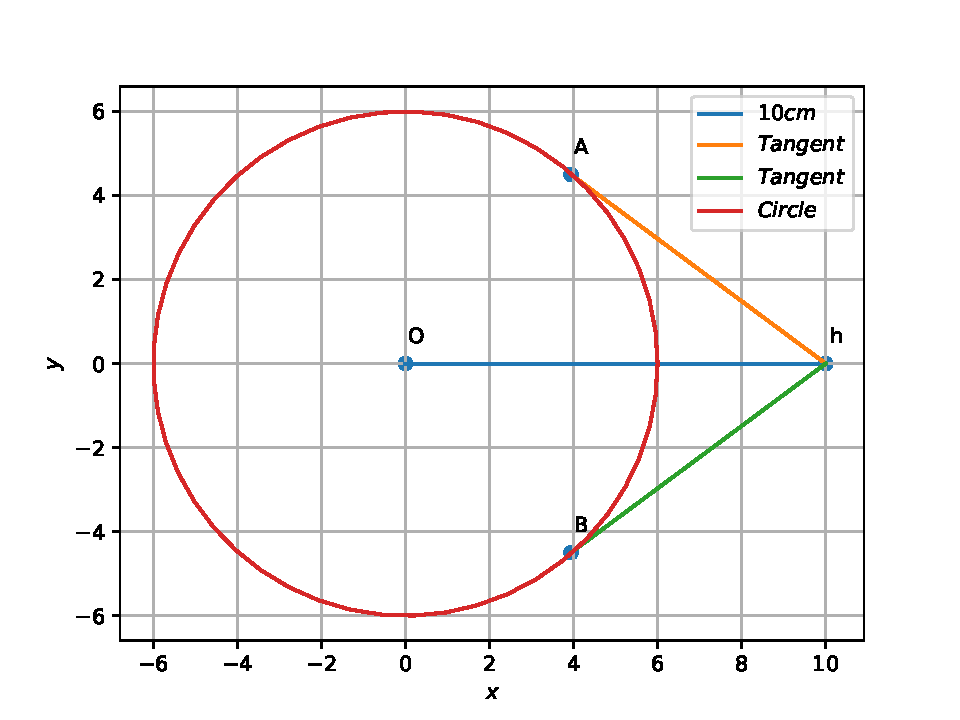
\includegraphics[width=1\columnwidth]{circle1.pdf}
\caption{Figure}
\label{fig:triangle}
\end{figure}

The dimensions of the figure is taken as below\\\\
{
\setlength\extrarowheight{2pt}
\centering
\begin{tabular}{|c|c|c|}
 \hline
 \textbf{Symbol}&\textbf{Value}&\textbf{Description}\\
 \hline
 r&6&Radius\\
 \hline
 h&10&distance\\
 \hline
 0&$d%
 \begin{pmatrix}
  cos(0)\\
  sin(0)\\
 \end{pmatrix}$%
 &centre\\
 \hline
 A&$a%
 \begin{pmatrix}
  cos\theta\\
  sin\theta\\
 \end{pmatrix}$%
 &point of contact\\
 \hline
 B&$b%
 \begin{pmatrix}
  cos\theta\\
  sin\theta\\
 \end{pmatrix}$%
 &point of contact\\
 \hline
\end{tabular}
}	
\\\\
	The equation of a conic with directrix $\vec{n^Tx}$ = c , eccentricity e anf focus $\boldsymbol{f}$ is given by
	
\begin{equation}
	\vec{x}^T\vec{V}\vec{x} + 2\vec{u}^T + f = 0
\end{equation}
	for circle eccentricity e = 0 then,\\
\begin{equation}
	\vec{V} = \vec{I} = \myvec{1&0\\0&1} , \vec{u} = \myvec{0\\0} , f = -r^2
\end{equation}
Point q on conic is given by 
\begin{equation}
	\vec{q} = \vec{V}^{-1}(\vec{n} - \vec{u})
\end{equation}
where, $\vec{n}$ is the normal vectors of the tangents from a point h to the conic are given by 
\begin{equation}
	\vec{n} = \frac{\vec{e_1}}{\vec{e_1^Th}} + \mu_i(\vec{Rh})
\end{equation}
\\
where $\mu _i$ 's are given by the following equation
\begin{equation}
	\mu_i = \frac{1}{\vec{{m^TVm}}}(\vec{-m^T(Vq+u)})	
\end{equation}
	 			$ \pm \sqrt{\vec{m^T(Vq+u)}^2 - (\vec{q^TVq + 2u^T} + f)(\vec{m^TVm)})}$
\\\\
$\mu _i$ 's are obtained by substituting the following in equation 6\\\\
\begin{equation}
	\vec{m} = (\vec{Rh})  ;  \vec{u}  = \myvec{0\\0}  ;  \vec{q} = \frac{\vec{e_1}}{\vec{e_1^Th}}
\end{equation}
 $\vec{R}$ = $\myvec{0&-1\\1&0}$ 
The obtained $\mu_i$'s are substituted in equation 5 and equation 5 is substituted in equation 6 the required points on conic A and B are obtained.\\\\
Now the point A and B are formed and tangents are drawn \\\\
To find the length of point h and point A \\
\begin{center}
	The distance between h and A is $\norm{\vec{h}-\vec{A}}$\\
\end{center}
\begin{equation}
  (\vec{h}-\vec{A})(\vec{h}-\vec{A})^T=d^2
\end{equation}
\begin{center}
	By solving  equation(7) we get \\
	    distance  d=$8cm$\\
	    \begin{equation}
  (\vec{h}-\vec{A})(\vec{h}-\vec{A})^T=d^2
\end{equation}
\end{center}
\begin{center}
	By solving  equation(7) we get \\
	    distance  d=$8cm$\\
	    \begin{equation}
	    \norm{\vec{h}-\vec{A}}=8cm
	    \end{equation}=8cm
\end{center}
To find the length of point h and point B\\
\begin{center}
	The distance between h and B is $\norm{\vec{h}-\vec{B}}$\\
\end{center}
\begin{equation}
  (\vec{h}-\vec{B})(\vec{h}-\vec{B})^T=d^2
\end{equation}
\begin{center}
	By solving  equation(10) we get \\
	    distance  d=$8cm$\\
	    \begin{equation}
	    \norm{\vec{h}-\vec{B}}=8cm
	    \end{equation}
	    from equation (9) and (11)\\
	    \begin{equation}
	    \norm{\vec{h}-\vec{A}}=\norm{\vec{h}-\vec{B}}
	    \end{equation}
	    \end{center}
	    Hence,the above equation (12) we can prove that the lenght of the tangents to a circle of radius 6cm,from a point 10cm away from the centre of the circle,is 8cm.\\
	    
	    
The below python code realizes the above construction:	\\
\begin{lstlisting}
https://github.com/soundaryanaru/FWC-assignments/blob/main/Matrix/circle_assignment/code/circle.py
\end{lstlisting}
\bibliographystyle{ieeetr}
\end{document}
